\documentclass[12pt,a4paper]{article}
\usepackage[utf8]{vietnam}
\usepackage{amsmath}
\usepackage{amsfonts}
\usepackage{xcolor}
\usepackage{titlesec}
\usepackage{mdframed}
\usepackage{amssymb}
\usepackage{pgf,tikz,pgfplots}
\usepackage{graphicx}
\usepackage{cases} 
\pgfplotsset{compat=1.5}
\usepackage{mathrsfs}
\usetikzlibrary{arrows, calc}
\usepackage{fancyhdr}
\pagestyle{fancy}
\pagestyle{empty}
\usepackage[left=2cm,right=2cm,top=2cm,bottom=2cm]{geometry}
\author{Nguyễn Văn Lộc}
\newmdenv[linecolor=black,skipabove=\topsep,skipbelow=\topsep,
leftmargin=-5pt,rightmargin=-5pt,
innerleftmargin=5pt,innerrightmargin=5pt]{mybox}
\begin{document}
\fancyhf{}
\lhead{}
\chead{}
\rhead{}
\cfoot{\thepage}
\rfoot{}
\lfoot{}
\pagestyle{fancy}
\renewcommand{\headrulewidth}{0pt}
\renewcommand{\footrulewidth}{0pt}
\begin{flushleft}
\begin{mybox}
\textbf{Họ và tên:} Nguyễn Văn Lộc\\
\textbf{MSSV:} 20120131\\ 
\textbf{Lớp:} 20CTT1TN\\
\textbf{Ca:} Ca 1 sáng thứ 4
\end{mybox}
\end{flushleft}
\begin{center}
\textbf{BÀI TẬP THỰC HÀNH VI TÍCH PHÂN 2B}\\
\textbf{CHƯƠNG 3: TÍCH PHÂN BỘI}
\end{center}
\textbf{Teang 52}\\
\textbf{Bài 15.}
\begin{mybox}
Tính tích phân kép  \(I = \int {\int_R {\left( {6{x^2}{y^3} - 5{y^4}} \right)dA} } \) với \(R = \left\{ {\left. {\left( {x,y} \right)} \right|0 \leqslant x \leqslant 3,0 \leqslant y \leqslant 1} \right\}.\)
\end{mybox}
\[I = \int\limits_0^3 {\int\limits_0^1 {\left( {6{x^2}{y^3} - 5{y^4}} \right)dydx = \int\limits_0^3 {\left( {\int\limits_0^1 {\left( {6{x^2}{y^3} - 5{y^4}} \right)dy} } \right)} } } dx\]
\[ = \int\limits_0^3 {\left( {\left. {\left( {\frac{3}{2}{x^2}{y^4} - {y^5}} \right)} \right|_{y = 0}^{y = 1}} \right)dx = \int\limits_0^3 {\left( {\frac{3}{2}{x^2} - 1} \right)dx = \left. {\left( {\frac{1}{2}{x^3} - x} \right)} \right|} } _{x = 0}^{x = 3} = \frac{{21}}{2}.\]
\textbf{Trang 53.}\\
\textbf{Bài 21.}
\begin{mybox}
Tính tích phân kép \(I = \int {\int_R {xy{e^{{x^2}y}}dA} } \) với \(R = \left[ {1,2} \right] \times \left[ {0,2} \right].\)
\end{mybox}
\[I = \int\limits_0^2 {\int\limits_1^2 {xy{e^{{x^2}y}}dx} } dy = \int\limits_0^2 {\left( {\int\limits_1^2 {xy{e^{{x^2}y}}dx} } \right)} dy\]
Đặt \(t = {x^2}y \Rightarrow dt = 2xydx.\)
\[ \Rightarrow \int {xy{e^{{x^2}y}}} dx = \frac{1}{2}\int {{e^t}dt = \frac{{{e^t}}}{2} + C = \frac{{{e^{{x^2}y}}}}{2}}  + C\]
\[ \Rightarrow I = \frac{1}{2}\int\limits_0^2 {\left( {\left. {\left( {{e^{{x^2}y}}} \right)} \right|_{x = 1}^{x = 2}} \right)dy = \frac{1}{2}} \int\limits_0^2 {\left( {{e^{4y}} - {e^y}} \right)} dy\]
\[ = \frac{1}{2}\left. {\left( {\frac{{{e^{4y}}}}{4} - {e^y}} \right)} \right|_{y = 0}^{y = 2} = \frac{{{e^8}}}{8} - \frac{{{e^2}}}{2} + \frac{3}{8}.\]
\textbf{Bài 28.} 
\begin{mybox}
Tính thể tích khối rắn được bao quanh bởi các mặt \(z = x{\sec ^2}y,\) \(z = 0,\) \(x = 0,\) \(x = 2,\) \(y = 0\) và \(y = \frac{\pi }{4}.\)
\end{mybox}
Thể tích cần tìm là:
\[V = \int\limits_0^2 {\int\limits_0^{\frac{\pi }{4}} {x{{\sec }^2}ydydx} } \]
\[ = \int\limits_0^2 {\left( {\int\limits_0^{\frac{\pi }{4}} {x{{\sec }^2}ydy} } \right)} dx = \int\limits_0^2 {\left( {\left. {\left( {x\tan y} \right)_{y = 0}^{y = \frac{\pi }{4}}} \right|} \right)} dx\]
\[ = \int\limits_0^2 {xdx}  = \left. {\frac{{{x^2}}}{2}} \right|_{x = 0}^{x = 2} = 2 \Rightarrow V = 2.\]
\textbf{Bài 30.}
\begin{mybox}
Tính thể tích khối rắn được bao bởi mặt paraboloid \(z = 2 + {x^2} + {\left( {y - 2} \right)^2}\) và các mặt phẳng \(z = 1,\) \(x = 1,\) \(x =  - 1,\) \(y = 0,\) \(y = 4.\)
\end{mybox}
Thể tích cần tìm là \(V = \left| I \right|,\) với \(I = \int\limits_{ - 1}^1 {\int\limits_0^4 {\left( {2 + {x^2} + {{\left( {y - 2} \right)}^2} - 1} \right)dydx} } .\)
\[I = \int\limits_{ - 1}^1 {\left( {\int\limits_0^4 {\left( {2 + {x^2} + {{\left( {y - 2} \right)}^2} - 1} \right)dy} } \right)dx = \int\limits_{ - 1}^1 {\left( {\int\limits_0^4 {\left( {{x^2} + {y^2} - 4y + 5} \right)dy} } \right)dx} } \]
\[ = \int\limits_{ - 1}^1 {\left( {\left. {\left( {{x^2}y + \frac{{{y^3}}}{3} - 2{y^2} + 5y} \right)} \right|_{y = 0}^{y = 4}} \right)} dx = \int\limits_{ - 1}^1 {\left( {4{x^2} + \frac{{28}}{3}} \right)} dx = \frac{{64}}{3}.\]
\[ \Rightarrow V = \frac{{64}}{3}.\]
\textbf{Trang 56}\\
\textbf{Bài 6.}
\begin{mybox}
Tính tích phân lặp \(I = \int {\int_D {{y^2}dA,} } \) với \(D = \left\{ {\left. {\left( {x,y} \right)} \right| - 1 \leqslant y \leqslant 1, - y - 2 \leqslant x \leqslant y} \right\}.\)
\end{mybox}
\[I = \int\limits_{ - 1}^1 {\int\limits_{ - y - 2}^y {{y^2}dxdy} }  = \int\limits_{ - 1}^1 {\left( {\int\limits_{ - y - 2}^y {{y^2}dx} } \right)dy} \]
\[ = \int\limits_{ - 1}^1 {\left( {\left. {\left( {x{y^2}} \right)} \right|_{x =  - y - 2}^{x = y}} \right)dy = \int\limits_{ - 1}^1 {\left( {2{y^3} + 2{y^2}} \right)dy = \frac{4}{3}} } .\]
\textbf{Bài 12.}
\begin{mybox}
Tính tích phân lặp \(I = \int {\int_D {x\cos ydA} }, \) với \(D\) là miền được bao bởi \(y = 0,\) \(y = {x^2},\) \(x = 1.\)
\end{mybox}
Xét phương trình hoành độ giao điểm
\[{x^2} = 0 \Leftrightarrow x = 0.\]
\[ \Rightarrow I = \int\limits_0^1 {\int\limits_0^{{x^2}} {x\cos ydydx} } \]
\[I = \int\limits_0^1 {\left( {\left. {\left( {x\sin y} \right)} \right|_{y = 0}^{y = {x^2}}} \right)}  = \int\limits_0^1 {x\sin \left( {{x^2}} \right)} dx\]
\[ = \left. {\left( { - \frac{1}{2}\cos \left( {{x^2}} \right)} \right)} \right|_{x = 0}^{x = 1} =  - \frac{1}{2}\cos \left( 1 \right) + \frac{1}{2}.\]
\textbf{Bài 13.}
\begin{mybox}
Tính tích phân lặp \(I = \int {\int_D {\left( {x + y} \right)dA} } ,\) với \(D\) là miền được bao bởi \(y = \sqrt x ,\) \(y = {x^2}.\)
\end{mybox}
Xét phương trình hoành độ giao điểm
\[{x^2} = \sqrt x  \Leftrightarrow \left[ \begin{gathered}
  x = 0 \hfill \\
  x = 1 \hfill \\ 
\end{gathered}  \right..\]
\[\forall x \in \left[ {0,1} \right],{x^2} \leqslant \sqrt x .\]
\[ \Rightarrow I = \int\limits_0^1 {\int\limits_{{x^2}}^{\sqrt x } {\left( {x + y} \right)dy} dx} .\]
\[I = \int\limits_0^1 {\int\limits_{{x^2}}^{\sqrt x } {\left( {x + y} \right)dy} dx}  = \int\limits_0^1 {\left( {\left( {xy + \frac{{{y^2}}}{2}} \right)_{y = {x^2}}^{y = \sqrt x }} \right)} dx\]
\[ = \int\limits_0^1 {\left( {x\sqrt x  + \frac{x}{2} - {x^3} - \frac{{{x^4}}}{2}} \right)} dx = \left. {\left( {\frac{2}{5}{x^2}\sqrt x  + \frac{{{x^2}}}{4} - \frac{{{x^4}}}{4} - \frac{{{x^5}}}{{10}}} \right)} \right|_{x = 0}^{x = 1} = \frac{3}{{10}}.\]
\textbf{Bài 14.}
\begin{mybox}
Tính tích phân lặp \(I = \int {\int_D {{y^3}} dA}, \) với \(D\) là miền hình tam giác với các đỉnh \(\left( {0,2} \right),\) \(\left( {1,1} \right),\) \(\left( {3,2} \right).\)
\end{mybox}
\definecolor{zzttqq}{rgb}{0.6,0.2,0}
\definecolor{ududff}{rgb}{0.30196078431372547,0.30196078431372547,1}
\begin{center}
\begin{tikzpicture}[line cap=round,line join=round,>=triangle 45,x=1cm,y=1cm]
\clip(-3.89736956534122,-1.0436861415133) rectangle (7.730793393766587,4.479211871748851);
\fill[line width=2pt,color=zzttqq,fill=zzttqq,fill opacity=0.10000000149011612] (0,2) -- (1,1) -- (3,2) -- cycle;
\draw [line width=2pt,color=zzttqq] (0,2)-- (1,1);
\draw [line width=2pt,color=zzttqq] (1,1)-- (3,2);
\draw [line width=2pt,color=zzttqq] (3,2)-- (0,2);
\draw [->, line width=2pt] (-3.89736956534122,0)--(7.730793393766587,0);
\draw [->, line width=2pt] (0,-1.0436861415133)--(0,4.479211871748851);
\begin{scriptsize}
\draw [fill=ududff] (0,2) circle (2.5pt);
\draw[color=ududff] (0.08473743212906168,2.2161845703514373) node {$A$};
\draw [fill=ududff] (1,1) circle (2.5pt);
\draw[color=ududff] (1.080264181496632,1.2206578209838674) node {$B$};
\draw (0,0) node [below right] {$O$};
\draw [fill=ududff] (1,0) circle (2.5pt);
\draw [fill=ududff] (0,1) circle (2.5pt);
\draw [fill=ududff] (2,0) circle (2.5pt);
\draw [fill=ududff] (3,0) circle (2.5pt);
\draw [fill=ududff] (3,2) circle (2.5pt);
\draw[color=ududff] (3.081580842596387,2.2161845703514373) node {$C$};
\draw[color=zzttqq] (0.4234217901613279,1.508026367193063) node [below left] {$b$};
\draw[color=zzttqq] (2.1065804179580447,1.4772368800992206) node [below right] {$a$};
\end{scriptsize}
\end{tikzpicture}
\end{center}
Đường thẳng \(BC\) có phương trình:
\[x - 2y + 1 = 0\]
\[ \Leftrightarrow x = 2y - 1.\]
Đường thẳng \(AB\) có phương trình: 
\[x + y - 2 = 0\]
\[ \Leftrightarrow x =  - y + 2.\]
\[ \Rightarrow I = \int\limits_1^2 {\int\limits_{ - y + 2}^{2y - 1} {{y^3}dxdy.} } \]
\[I = \int\limits_1^2 {\int\limits_{ - y + 2}^{2y - 1} {{y^3}dxdy}  = \int\limits_1^2 {\left( {\left. {\left( {x{y^3}} \right)} \right|_{x =  - y + 2}^{x = 2y - 1}} \right)dy} } \]
\[ = \int\limits_1^2 {\left( {3{y^4} - 3{y^3}} \right)} dy = \frac{{147}}{{20}}.\]
\textbf{Bài 21.}
\begin{mybox}
Tính thể tích khối rắn được bao bởi paraboloid \(z = x^2 + 3y^3\) và mặt \(x = 0, y = 1, y = x, z = 0.\)
\end{mybox}
Thể tích cần tìm là \(V = \left| I \right|,\) với \(I = \int\limits_0^1 {\int\limits_x^1 {\left( {{x^2} + 3{y^3}} \right)} } dydx.\)
\[I = \int\limits_0^1 {\left( {\left. {\left( {{x^2}y + \frac{{3{y^4}}}{4}} \right)} \right|_{y = x}^{y = 1}} \right)dx = \int\limits_0^1 {\left( {{x^2} + \frac{3}{4} - {x^3} - \frac{{3{y^4}}}{4}} \right)} } dx = \frac{{41}}{{60}}.\]
\textbf{Bài 23.}
\begin{mybox}
Tính thể tích khối rắn tạo bởi các mặt phẳng \(z = x,\) \(y = x,\) \(x + y = 2,\) và \(z = 0.\)
\end{mybox}
\definecolor{zzttqq}{rgb}{0.6,0.2,0}
\definecolor{xdxdff}{rgb}{0.49019607843137253,0.49019607843137253,1}
\definecolor{uuuuuu}{rgb}{0.26666666666666666,0.26666666666666666,0.26666666666666666}
\begin{center}
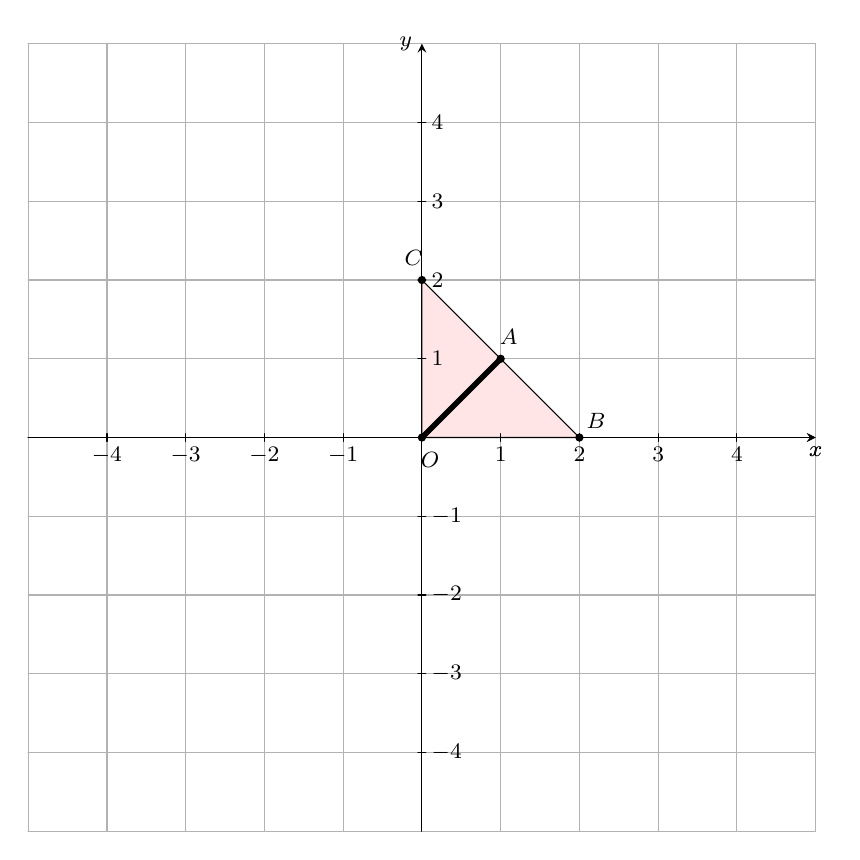
\begin{tikzpicture}[line join = round, line cap = round,>=stealth,font=\footnotesize,scale=1]
\path
(0,0) coordinate (O)
(0,2) coordinate (C)
(2,0) coordinate (B)
(1,1) coordinate (A)
;
\draw[opacity=0.3] (-5,-5) grid (5,5) ;
\draw[fill=red!10]
(O)--(B)--(C)--cycle
;
\draw [line width=2pt] (O)--(A);
\draw[->](-5,0)--(5,0) node [below] {$x$};
\draw[->](0,-5)--(0,5)node [left] {$y$};
\foreach \y in {-4,...,-1,1,2,...,4}
{\draw ([xshift=-0.5mm]0,\y)--([xshift=0.5mm]0,\y) (0,\y) node[right]{$\y$};}
\draw[->] (-5,0)--(5,0)node[below]{$x$};
\foreach \x in {-4,...,-1,1,2,...,4}
{\draw ([yshift=-0.5mm]\x,0)--([yshift=0.5mm]\x,0) (\x,0) node[below]{$\x$};}
\foreach \x/\goc in {O/-70,A/70,B/45,C/110}
{\fill[black] (\x) circle (1.5pt) ($(\x)+(\goc:3mm)$) node{$\x$};}
\end{tikzpicture}
\end{center}
Đường thẳng \(OA\) có phương trình \(y = x.\)\\
Đường thẳng \(AB\) có phương trình \(x + y = 2 \Leftrightarrow y = 2 - x.\)\\
Dựa vào hình vẽ, ta được \(V = \int {\int_D {xdA,} } \) với \(D\) là miền thỏa mãn \(D = \left\{ {\left. {\left( {x,y} \right)} \right|0 \leqslant x \leqslant 1,x \leqslant y \leqslant 2 - x} \right\}.\)
Từ đó,
\[V = \int\limits_0^1 {\int\limits_x^{2 - x} {xdydx} }  = \int\limits_0^1 {\left( {\left. {\left( {xy} \right)} \right|_{y = x}^{y = 2 - x}} \right)} dx\]
\[ = \int\limits_0^1 {\left( {2x - 2{x^2}} \right)} dx = \frac{1}{3}.\]
\textbf{Trang 60.}\\
\textbf{Bài 9.}
\begin{mybox}
Tính tích phân \(I = \int {\int_R {\cos \left( {{x^2} + {y^2}} \right)} } dA,\) với \(R\) là miền nằm dưới trục \(Ox\) và bên trong đường tròn \(x^2 + y^2 = 9\) bằng cách đổi hệ tọa độ cực.
\end{mybox}
\begin{center}
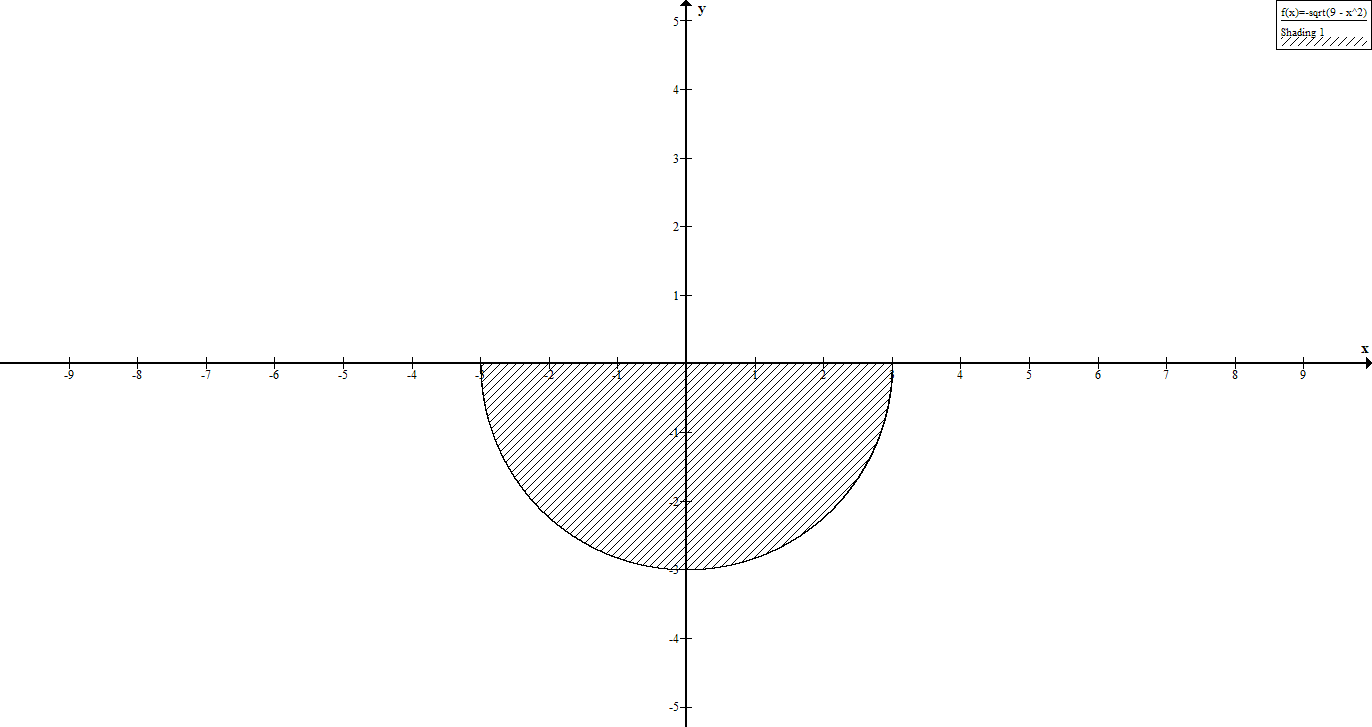
\includegraphics[scale=0.3]{c3_1}
\end{center}
Ta viết lại miền \(R\) như sau: 
\[R = \left\{ {\left. {\left( {r,\theta } \right)} \right|0 \leqslant r \leqslant 3, - \pi  \leqslant \theta  \leqslant 0} \right\}.\]
\[ \Rightarrow I = \int\limits_{ - \pi }^0 {\int\limits_0^3 {\cos \left( {{r^2}{{\cos }^2}\theta  + {r^2}{{\sin }^2}\theta } \right)rdrd\theta } } \]
\[ \Rightarrow I = \int\limits_{ - \pi }^0 {\int\limits_0^3 {\cos \left( {{r^2}} \right)rdrd\theta } }  = \int\limits_{ - \pi }^0 {\left. {\left( {\frac{1}{2}\sin \left( {{r^2}} \right)} \right)} \right|} _{r = 0}^{r = 3}d\theta \]
\[ \Rightarrow I = \int\limits_{ - \pi }^0 {\frac{{\sin 9}}{2}} d\theta  = \theta  \cdot \left. {\frac{{\sin 9}}{2}} \right|_{\theta  =  - \pi }^{\theta  = 0} = \frac{{\pi \sin 9}}{2}.\]
\textbf{Bài 11.}
\begin{mybox}
Tính tích phân \(I = \int {\int_R {y{e^x}} } dA,\) với \(R\) là miền nằm dưới trục \(Ox\) và bên trong đường tròn \(I = \int {\int_R {y{e^x}} } dA\) bằng phương pháp đổi hệ tọa độ cực.
\end{mybox}
\begin{center}
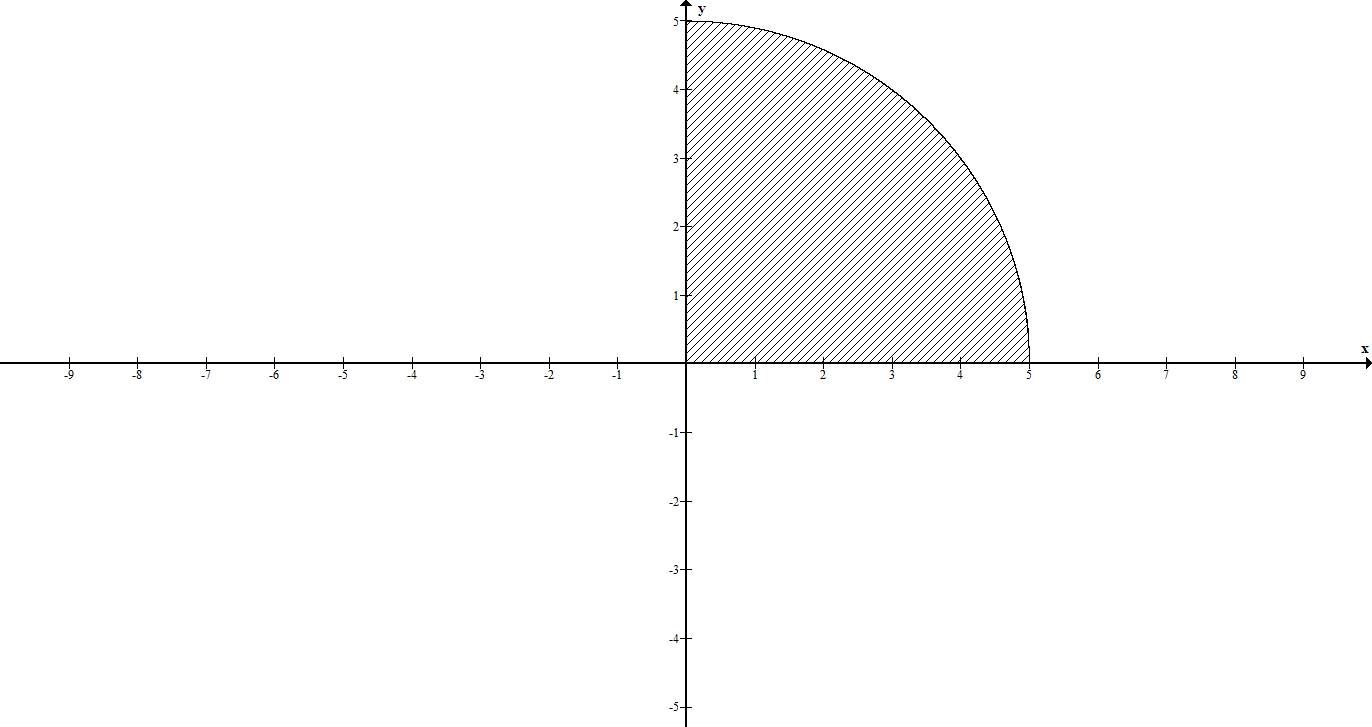
\includegraphics[scale=0.3]{c3_2}
\end{center}
Ta viết lại miền \(R\) như sau:
\[R = \left\{ {\left. {\left( {r,\theta } \right)} \right|0 \leqslant r \leqslant 5,0 \leqslant \theta  \leqslant \frac{\pi }{2}} \right\}.\]
\[ \Rightarrow I = \int\limits_0^{\frac{\pi }{2}} {\int\limits_0^5 {r\sin \theta {e^{r\cos \theta }}} } rdrd\theta \]
\[ \Rightarrow I = \int\limits_0^{\frac{\pi }{2}} {\int\limits_0^5 {{r^2}\sin \theta {e^{r\cos \theta }}} } drd\theta  = \int\limits_0^5 {\int\limits_0^{\frac{\pi }{2}} {{r^2}\sin \theta {e^{r\cos \theta }}d\theta dr} } \]
\[ \Rightarrow I = \int\limits_0^5 {\left. {\left( { - r{e^{r\cos \theta }}} \right)} \right|} _{\theta  = 0}^{\theta  = \frac{\pi }{2}}dr = \int\limits_0^5 {\left( { - r + r{e^r}} \right)} dr\]
\[ \Rightarrow I = \left. {\left( { - \frac{{{r^2}}}{2} + \left( {r - 1} \right){e^r}} \right)} \right|_{r = 0}^{r = 5} = 4{e^5} - \frac{{23}}{2}.\]
\end{document}